% Wissenswertes:
% \todo und \missingfigure erzeugen eine Warning: bad box, Underfill ... -> diese kann ignoriert werden

\documentclass[fontsize=12pt, a4paper, headinclude, twoside=false, parskip=half+, pagesize=auto, numbers=noenddot, plainheadsepline, open=right, toc=listof, toc=bibliography, chapteratlists=0pt]{scrartcl}

% Allgemeines
\usepackage{scrlayer-scrpage} % Kopf- und Fußzeilen
\usepackage{amsmath,marvosym} % Mathesachen
\usepackage[T1]{fontenc} % Ligaturen, richtige Umlaute im PDF
\usepackage[utf8]{inputenc}% UTF8-Kodierung für Umlaute usw
\usepackage{caption}
\usepackage[Q=yes]{examplep}
\usepackage[colorinlistoftodos, textwidth=\marginparwidth]{todonotes}
\let\oldmissingfigure\missingfigure % save old command
\renewcommand{\missingfigure}[1]{\oldmissingfigure[figwidth=\textwidth-2pt]{#1}}% renew \missingfigure command
\usepackage{geometry}
\geometry{
	left = 30mm,
	right = 30mm,
	top = 28mm,
}
%\usepackage{showframe} %Zeigt Rahmen um alle Objekte an

% Titelseite
\usepackage{titling}  % Sorgt für einen Titel und Inhalt auf selber Seite

% Schriften
\usepackage{setspace} % Zeilenabstand
\onehalfspacing % 1,5 Zeilen
\usepackage{lmodern}

% Schriften-Größen
\setkomafont{section}{\Large\rmfamily}
\setkomafont{subsection}{\large\rmfamily}
\setkomafont{subsubsection}{\small\rmfamily}
\setkomafont{descriptionlabel}{\bfseries\rmfamily} % für description Umgebungen
\setkomafont{captionlabel}{\small\bfseries}
\setkomafont{caption}{\small}

% Sprache: Deutsch
\usepackage[ngerman]{babel} % Silbentrennung

% PDF
\usepackage[ngerman, breaklinks=true]{hyperref}
\usepackage[final]{microtype} % mikrotypographische Optimierungen
\usepackage{url}
\usepackage{pdflscape} % einzelne Seiten drehen können

% Tabellen
\usepackage{multirow} % Tabellen-Zellen über mehrere Zeilen
\usepackage{multicol} % mehre Spalten auf eine Seite
\usepackage{tabularx} % Für Tabellen mit vorgegeben Größen
\usepackage{longtable} % Tabellen über mehrere Seiten
\usepackage{array}
\usepackage{float}
\usepackage{booktabs}

% Bibliographie / Quellenverzeichnis
\usepackage{bibgerm} % Umlaute in BibTeX
\usepackage[style=alphabetic]{biblatex} % Quellenverzeichnis und Zitate
\addbibresource{bibliographie.bib}

% Bilder
\usepackage{graphicx} % Bilder
\graphicspath{{images/}}
\DeclareGraphicsExtensions{.pdf,.png,.jpg} % bevorzuge pdf-Dateien
\usepackage[all]{hypcap} % Beim Klicken auf Links zum Bild und nicht zu Caption gehen


% Bildunterschrift
\usepackage{caption}
\usepackage{chngcntr}
\setcapindent{0em} % kein Einrücken der Caption von Figures und Tabellen
\setlength{\abovecaptionskip}{0.2cm} % Abstand der zwischen Bild- und Bildunterschrift

% Custom colors
\definecolor{deepblue}{rgb}{0,0,0.5}
\definecolor{purple}{rgb}{0.96,0.15,0.44}
\definecolor{deepgreen}{rgb}{0,0.5,0}
\definecolor{codegreen}{rgb}{0,0.6,0}
\definecolor{codegray}{rgb}{0.4,0.4,0.4}
\definecolor{codeblue}{rgb}{0.16,0.32,0.75}
\definecolor{backcolour}{rgb}{0.95,0.95,0.92}
\definecolor{codeorange}{rgb}{1.0,0.49,0.0}

% Quellcode
\usepackage{listings} % für Formatierung in Quelltexten
\usepackage{color}
\lstdefinestyle{mystyle}{
	backgroundcolor=\color{backcolour},
	commentstyle=\color{codegray},
	keywordstyle=\color{purple},
	emph={instr,import},
	emphstyle={\color{codeorange}},
	numberstyle=\tiny\color{codegray},
	stringstyle=\color{codeblue},
	basicstyle=\footnotesize,
	breakatwhitespace=false,
	breaklines=true,
	captionpos=b,
	keepspaces=true,
	numbers=left,
	numbersep=10pt,
	showspaces=false,
	showstringspaces=false,
	showtabs=false,
	tabsize=2,
	otherkeywords={vec4},
	morekeywords={vec4},
	frame=single,
	framerule=2pt,
	rulecolor=\color{backcolour},
}
\lstset{style=mystyle,language=Python}

% Eigene Befehle %%%%%%%%%%%%%%%%%%%%%%%%%%%%%%%%%%%%%%%%%%%%%%%%%
\newcommand{\image}[4][!h]{
	\begin{figure}[#1]
		\centering
		\vspace{1ex}
		\includegraphics[#3]{images/#2}
		\caption[#4]{#4}\label{img.#2}      
		\vspace{1ex}
	\end{figure}
}
 % Importiere die Einstellungen aus der Präambel

\pretitle{%
	\begin{center}
		\vspace{-25mm}
		\LARGE
		\hfill
\includegraphics[height=0.1\textwidth]{logo.png}\\[\bigskipamount]
		\vspace{10mm}
}
\posttitle{\end{center}}

\begin{document} % hier beginnt der eigentliche Inhalt
\pagestyle{scrheadings}
\chead{\headmark} % Kopfzeile, mittig
\overfullrule=3pt

% Titelseite ########################################################################################

\title{\textbf{Headline} \\ 
	\begin{small}
		\vspace{3mm}
		Modularbeit im Kurs \textit{Musterkurs} bei Prof. Dr. Max Mustermann\\
		\vspace{3mm}		
		Martin Musterstudent \\
		\textit{Fakultät für Mathematik und Informatik} \\
		\textit{Hochschule für angewandte Wissenschaften München}\\
		musterstudent@hm.edu \\
	\end{small}
}

\date{}

\maketitle


% Hier beginnt der Text: #####################################################

\vspace{-40mm}

\section{Auflistungen}

\subsection{Auflistungen}


\begin{itemize}
	\item Erster Punkt
	\item Zweiter Punkt der Auflistung
	\item Dritter ganz wichtiger Punkt
\end{itemize}

Und hier kommt etwas Blindtext. Lorem ipsum dolor sit amet, consectetuer adipiscing elit. Aenean commodo ligula eget dolor. Aenean massa. Cum sociis natoque penatibus et magnis dis parturient montes, nascetur ridiculus mus. Donec quam felis, ultricies nec, pellentesque eu, pretium quis, sem. Nulla consequat massa quis enim. Donec pede justo, fringilla vel, aliquet nec, vulputate eget, arcu. In enim justo, rhoncus ut, imperdiet a, venenatis vitae, justo. Nullam dictum felis eu pede mollis pretium. Integer tincidunt. Cras dapibus. Vivamus elementum semper nisi. Aenean vulputate eleifend tellus. Aenean leo ligula, porttitor eu, consequat vitae, eleifend ac, enim. Aliquam lorem ante, dapibus in, viverra quis, feugiat a, tellus. Phasellus viverra nulla ut metus varius laoreet. Quisque rutrum. Aenean imperdiet. Etiam ultricies nisi vel augue. Curabitur ullamcorper ultricies nisi. Nam eget dui. Etiam rhoncus. Maecenas tempus, tellus eget condimentum rhoncus, sem quam semper libero, sit amet adipiscing sem neque sed ipsum. Nam quam nunc, blandit vel, luctus pulvinar, hendrerit id, lorem. Maecenas nec odio et ante tincidunt tempus. Donec vitae sapien ut libero venenatis faucibus. Nullam quis ante. Etiam sit amet orci eget eros faucibus tincidunt. Duis leo. Sed fringilla mauris sit amet nibh. Donec sodales sagittis magna. Sed consequat, leo eget bibendum sodales, augue velit cursus nunc, quis gravida magna mi a libero. 

Fusce vulputate eleifend sapien. Vestibulum purus quam, scelerisque ut, mollis sed, nonummy id, metus. Nullam accumsan lorem in dui. Cras ultricies mi eu turpis hendrerit fringilla. Vestibulum ante ipsum primis in faucibus orci luctus et ultrices posuere cubilia Curae; In ac dui quis mi consectetuer lacinia. Nam pretium turpis et arcu. Duis arcu tortor, suscipit eget, imperdiet nec, imperdiet iaculis, ipsum. Sed aliquam ultrices mauris. Integer ante arcu, accumsan a, consectetuer eget, posuere ut, mauris. Praesent adipiscing. Phasellus ullamcorper ipsum rutrum nunc. Nunc nonummy metus. Vestibulum volutpat pretium libero. Cras id dui. Aenean ut eros et nisl sagittis vestibulum. Nullam nulla eros, ultricies sit amet, nonummy id, imperdiet feugiat, pede. Sed lectus. Donec mollis hendrerit risus. Phasellus nec sem in justo pellentesque facilisis. Etiam imperdiet imperdiet orci. Nunc nec neque. Phasellus leo dolor, tempus non, auctor et, hendrerit quis, nisi. Curabitur ligula sapien, tincidunt non, euismod vitae, posuere imperdiet, leo. Maecenas malesuada. Praesent congue erat at massa. Sed cursus turpis vitae tortor \cite{kurose_computernetzwerke:_2014}. 

Donec posuere vulputate arcu. Phasellus accumsan cursus velit. Vestibulum ante ipsum primis in faucibus orci luctus et ultrices posuere cubilia Curae; Sed aliquam, nisi quis porttitor congue, elit erat euismod orci, ac placerat dolor lectus quis orci. Phasellus consectetuer vestibulum elit. Aenean tellus metus, bibendum sed, posuere ac, mattis non, nunc. Vestibulum fringilla pede sit amet augue. In turpis. Pellentesque posuere. Praesent turpis. Aenean posuere, tortor sed cursus feugiat, nunc augue blandit nunc, eu sollicitudin urna dolor sagittis lacus. Donec elit libero, sodales nec, volutpat a, suscipit non, turpis. Nullam sagittis. Suspendisse pulvinar, augue ac venenatis condimentum, sem libero volutpat nibh, nec pellentesque velit pede quis nunc. Vestibulum ante ipsum primis in faucibus orci luctus et ultrices posuere cubilia Curae; Fusce id purus. Ut varius tincidunt libero. Phasellus dolor. Maecenas vestibulum mollis diam. Pellentesque ut neque. Pellentesque habitant morbi tristique senectus et netus et malesuada fames ac turpis egestas. In dui magna, posuere eget, vestibulum et, tempor auctor, justo. In ac felis quis tortor malesuada pretium. Pellentesque auctor neque nec urna. Proin sapien ipsum, porta a, auctor quis, euismod ut, mi. Aenean viverra rhoncus pede. Pellentesque habitant morbi tristique senectus et netus et malesuada fames ac turpis egestas. Ut non enim eleifend felis pretium feugiat. Vivamus quis mi. Phasellus a est. Phasellus magna. In hac habitasse platea dictumst. Curabitur at lacus ac velit ornare lobortis. Curabitur a felis in nunc fringilla tristique. Morbi mattis ullamcorper velit. Phasellus gravida semper nisi. Nullam vel sem. Pellentesque libero tortor, tincidunt et, tincidunt eget, semper nec, quam. Sed hendrerit. Morbi ac felis \cite{guttich_intrusion-detection_2018}.


\section{Tabellen}

\begin{table}[!hbt]
	\begin{center}
		\begin{tabular}{ l c }
			\toprule
			\textbf{Modul} & \textbf{Durchschnittslaufzeit in Sekunden}\\
			\midrule   
			DNSresolver            & 0,314 \\
			DomainAge               & 0,495 \\
			GeoIP                   & 2,195 \\
			GoogleSafeBrowsingAPI   & 0,145 \\
			GoogleSearch            & 1,349 \\
			Nmap                    & 4,836 \\
			RobotsTxt               & 0,284 \\
			Traceroute              & 10,026 \\
			Typo                    & 0,583 \\
			Whois                   & 0,166 \\
			\midrule
			\textbf{Alle Module}    & \textbf{10,043} \\
			\bottomrule
		\end{tabular}
		\caption{Laufzeiten der einzelnen Module}\label{tab.laufzeit}
	\end{center}
\end{table}


\begin{figure}[!hbt]
	\begin{minipage}[!hbt]{5cm}
		\centering
		
		\begin{tabular}{l|c}
			\toprule
			\textbf{Anzahl Threads} & \textbf{Laufzeit in s} \\
			\midrule
			Sequenziell & 531,27 \\
			2 & 260,67 \\
			5 & 106,77 \\
			10 & 69,02 \\
			15 & 70,53 \\
			20 & 66,48 \\
			50 & 62,94 \\
			\bottomrule
		\end{tabular}
		
	\end{minipage}
	\hfill
	\begin{minipage}[!hbt]{8.2cm}
		\centering
	
		
			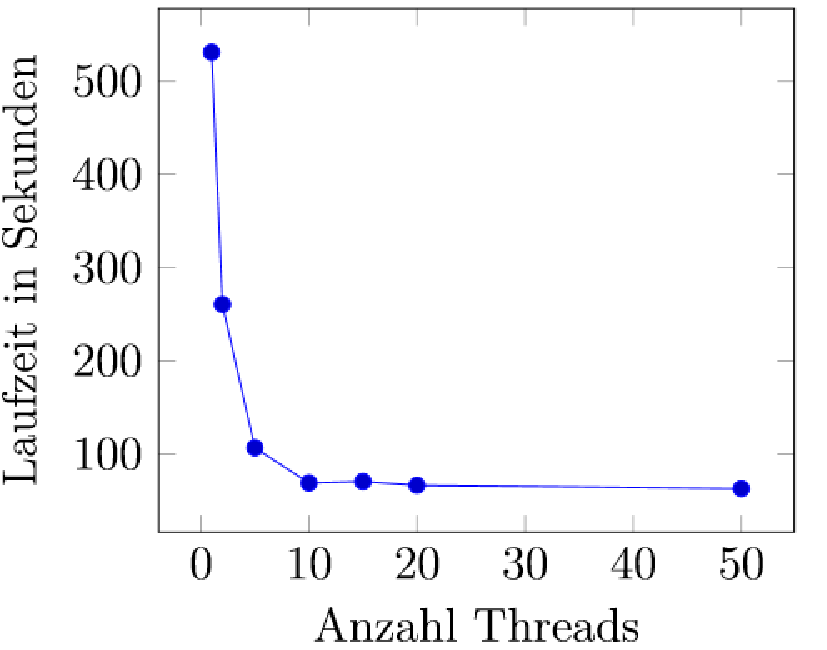
\includegraphics[scale=0.6]{images/laufzeiten}			 
		
	\end{minipage}
	\caption{Anzahl der Threads im Verhältnis zu Laufzeit}\label{fig.laufzeitListe}
\end{figure}

% Quellenverzeichnis: ##############################################################################

% Für die Zitate verwende ich BiLaTeX mit Alphabetischem Stil (statt numeric)
% Das Quellen- oder Literaturverzeichnis ist in zwei separate Listen aufgeteilt:
% - Bücher
% - Sonstige Quellen
% Vor dem Einbinden, muss Biber auf die Thesis angewendet werden:
% $ biber thesis
% ACHTUNG: <thesis> OHNE DATEIENDUNG!
% Erst danach koennen die Zitate verwendet werden!!!!

\section*{Quellenverzeichnis}
\addcontentsline{toc}{chapter}{Quellenverzeichnis}
\printbibliography[type=book,heading=subbibliography,title={Bücher}]
\printbibliography[nottype=book,heading=subbibliography,title={Sonstige Quellen}]

\end{document}
